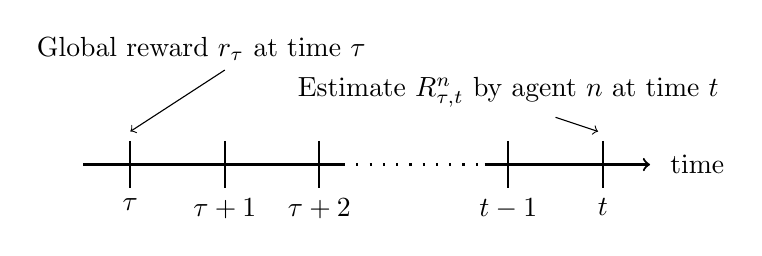
\begin{tikzpicture}[scale=0.6] % Smaller scale

    % Timeline with arrow
    \draw[black,thick, -] (-2.5,0) -- (3,0);
    \draw[black,thick, ->] (6,0) -- (9.5,0); % Horizontal line with arrow at the end

    % Markers with labels
    \draw[thick,black] (-1.5,0.5) -- (-1.5,-0.5) node[below] {$\tau$};
    \draw[thick,black] (0.5,0.5) -- (0.5,-0.5) node[below] {$\tau+1$};
    \draw[thick,black] (2.5,0.5) -- (2.5,-0.5) node[below] {$\tau+2$};

    % Dotted line for the break between $\tau+2$ and $T-1$
    \draw[loosely dotted,thick,black] (3,0) -- (6,0); % Dotted line between tau+2 and T-1

    % More markers and labels
    \draw[thick,black] (6.5,0.5) -- (6.5,-0.5) node[below] {$t-1$};
    \draw[thick,black] (8.5,0.5) -- (8.5,-0.5) node[below] {$t$};


    \node[above] at (0,2) {Global reward $r_\tau$ at time $\tau $};
    \draw[->] (0.5,2) -- (-1.5,0.7) ;

    % Agent n above T
    \node[above] at (6.5,1) {Estimate $R^n_{\tau,t}$ by agent $n$ at time $t$};
    \draw[->] (7.5,1) -- (8.4,0.7) ;

    % Arrow pointing to the end, with label t
    \node at (10.5,0) {time}; % Label 'time' at the end
    %\draw[thick, ->] (9, 0) -- (9.5, 0); % Arrow pointing to the right to indicate end
    
\end{tikzpicture}
